\subsection{Módulo MP3}
El modelo de MP3 seleccionado ha sido el YX5300, el cual se muestra en la \autoref{fig:2-3-MP3}.

Este reproductor se comunica con el microcontrolador mediante UART, con una velocidad de 9600 bps. También cuenta con una frecuencia de muestreo de 48 kHz y soporta tanto el formato MP3 como el formato WAV. Este modelo cuenta con un socket de tarjeta microSD en la cual se introducen las canciones, en los formatos antes mencionados, que se deseen reproducir. Dicha tarjeta deberá estar en formato Fat16 o Fat32 y tener como máximo \texttt{2 GB} de almacenamiento.

En cuento a la señal de audio obtenida a la salida del reproductor, podemos observar una salida bipolar entrada en 0V. Este comportamiento es totalmente inesperado ya que, al estar alimentado entre 3.3V y 0V, es extraño que la señal de salida pueda presentar valores negativos. Esto ha supuesto un gran problema en la unificación con el resto de módulos. Dicho problema y su solución será comentada en el \autoref{subsec:entre-dos-tierras}.

Por otra parte, el reproductor debe ser alimentadocon una tensión entre 3.2V y 5.2V, soporta una corriente máxima de 200mA y cuenta con un LED rojo que indica si está reproduciendo alguna canción.

Todas las características del reproductor MP3 se han obtenido del datasheet ofrecido por el fabricante. \cite{Catalex_MP3_boardPdf}

\begin{figure}[h]
    \centering
    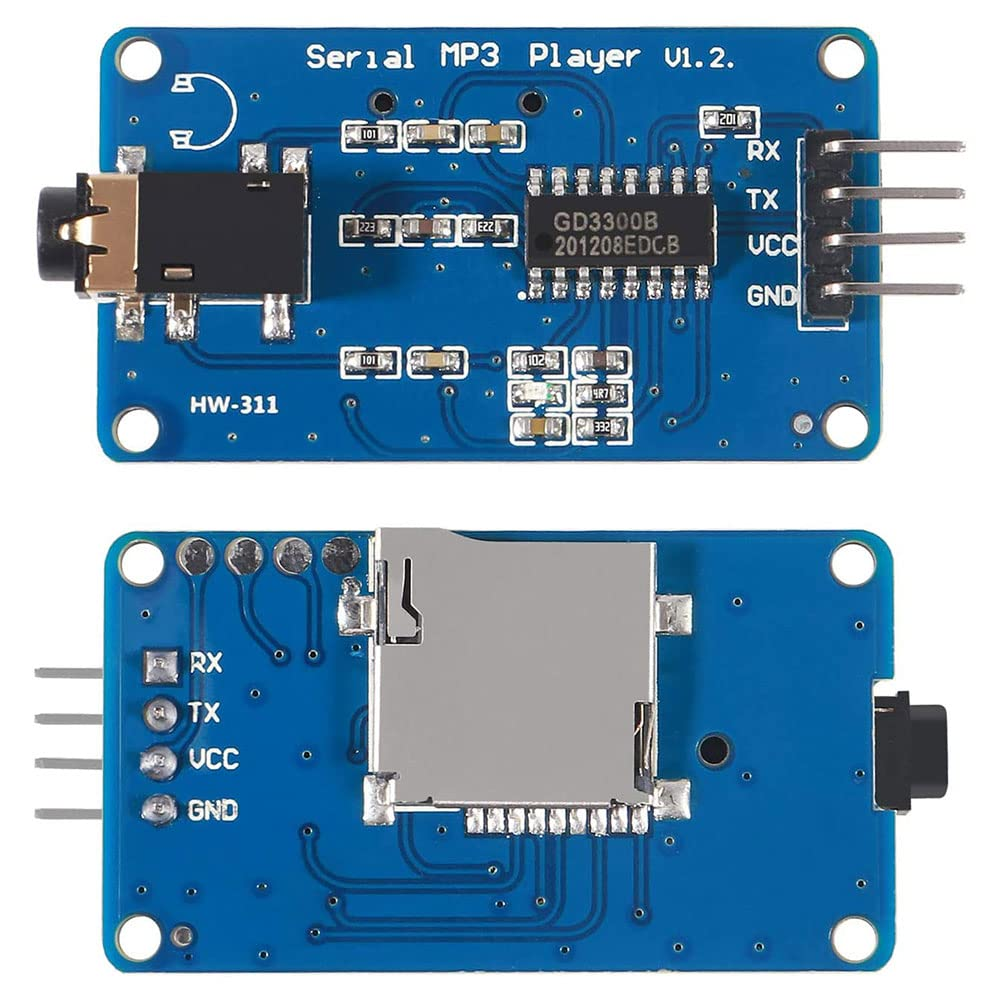
\includegraphics[width=0.3\textwidth]{images/2/2-4/MP3.jpg}
    \caption{Reproductor MP3 YX5300}
    \label{fig:2-3-MP3}
\end{figure}